\documentclass[12pt, a4paper, oneside]{ctexart}
\usepackage{amsmath, amsthm, amssymb, bm, color, framed, graphicx, hyperref, mathrsfs}

\title{\textbf{计算机程序设计 2025秋 USTC}}
\author{姓名:石泊远$ \hspace{1cm} $学号:PB25000051}
\date{\today}
\linespread{1.5}
\definecolor{shadecolor}{RGB}{241, 241, 255}
\newcounter{problemname}
\newenvironment{problem}{\begin{shaded}\stepcounter{problemname}\par\noindent\textbf{Assignments ~ \arabic{problemname}. }}{\end{shaded}\par}
\newenvironment{solution}{\par\noindent\textbf{Answer. }}{\par}
\newenvironment{note}{\par\noindent\textbf{Assignments ~ \arabic{problemname}'s Remark. }}{\par}
\newenvironment{remark}{\noindent \textbf{Remark.}}{}

\begin{document}
	%Introduction
	\maketitle
	
	%main body
	\begin{problem}
		了解三进制与三进制计算机的优缺点
	\end{problem}
	
	\begin{solution}
		三进制有两种计数体系:正常三进制$(0,1,2)$和平衡三进制$(-1,0,1)$ \\
		由于将$-1$写成数字不方便,我们将它记为Z,该计数体系的优点是负数表示容易,只需将正数的数字倒转即可\\ \\
		三进制更符合人类思维模式与人工智能的学习方式,同时在描述数字上较二进制也有效率更高的优点,但为什么我们现在没能使用三进制电脑呢? \\
		一是因为二进制只需要识别两种电压,可以使用二极管来实现,但三进制的表示需要三种稳定的材料,就算有了,稳定性也肯定不如二进制高,故我们现在使用的是二进制 \\
	\end{solution}
	
	\begin{problem}
		了解移码的原理以及更多浮点数的存储细节,并思考为什么一些标准的指数部分和尾数部分分别采用这两种编码方式 \\
	\end{problem}
	
	\begin{solution}
		移码:在移码中,全部的数都被加上一个基准偏移值,这个偏移值是一个根据场景限制选择的固定整数,保证要表示的负数都在相加后变成某个范围内的数(通常是无符号数范围),也就可以保证计算机中的$0$为全零,然后按照偏移过的数表示为二进制。 \\ \\
		浮点数的存储细节这里参考IEEE 754和深入理解计算机系统 (Randal E. Bryant, David R. O’Hallaron) (Z-Library)\\
		IEEE 754规定了四种表示浮点数值的方式:单精确度(32位)、双精确度(64位)、延伸单精确度(43比特以上,很少使用)与延伸双精确度(79比特以上,通常以80位实现)。只有32位模式有强制要求,其他都是选择性的。大部分编程语言都提供了IEEE浮点数格式与算术,但有些将其列为非必需的。例如,IEEE 754问世之前就有的C语言,现在包括了IEEE算术,但不算作强制要求(C语言的float通常是指IEEE单精确度,而double是指双精确度)。 \\
		一个浮点数的表示其实可被改写为这样: 
		$$ \bm{Value = sign \times exponent \times fraction} $$
		也就是一个浮点数的实际值等于符号位$*$指数偏移值$*$分数值 \\
		通过https://www.h-schmidt.net/FloatConverter/IEEE754.html,我们可以理解他的构造 \\
		指数部分会减去$127$后放在$2$的幂次上,尾数部分最高位代表$0.5$,后面以此类推可得 \\
		%%
		但也存在一些其他的概念,下面列举 \\
		\Large 概念1: normal number(规格数) 与 subnormal number(非规格数) \\
		\normalsize 根据IEEE754的规定, 按照尾数位隐藏的整数部分是 1。还是0. 可以将浮点数划分为两类: normal number(规格数) 和 subnormal number(非规格数)\\
		下面以32位浮点数为例来解释这些概念.\\
		\textbf{normal number(规格数)}就是尾数位隐藏的整数部分是1.的数, 可以理解为"正常的数",一般来说, 我们遇到的都是normal number \\
		举例: 20.5在内存中表示为:$ 0~1000~0011~\bm{0100}~\bm{1000}~\bm{0000}~\bm{0000}~\bm{000} $ \\
		其中尾数部分(即上面的加粗部分), 去掉后面补的零之后为: 01001,但事实上, 真实的尾数部分应该是: 1.01001, 即前面省略了整数部分1. \\
		\textbf{subnormal number(非规格数)}就是尾数位隐藏的整数部分为0.的数, 也叫作denormal number, 可以理解为"低于正常数的数"\\
		引入subnormal number这个概念, 是为了在浮点数下溢时, 可以逐位的损失精度, 以尽可能精确的表达0附近的极小数 \\
		为了表示subnormal number, IEEE754规定: 如果将指数位全部填充为0, 则表示这个数是个subnormal number\\
		举例: 以32位浮点数为例, 当你看到类似于 * 00000000 *********************** 这样内存状态的数时, (即指数位全部为0的数), 就应该知道, 这是个subnormal number, 此时这个数的尾数位隐藏的整数不是1. 而是0. \\
		\Large 概念2: non-number(特殊数) \\
		\normalsize 和subnormal number类似, IEEE754对于指数位全为1的状态也做了特殊规定:当指数位全部被1填充, 即指数位表示的值为255时, 用于表示这个浮点数处在一种非正常数(non-number)的状态: 即这个数可能是±infinity或NaN. \\
		所以: 当你看到类似于 * 11111111 *********************** 这样内存状态的数时, (即指数位全部为1的数), 就应该知道, 这是个non-number, 它用于表示特殊数. \\
		\begin{center}
			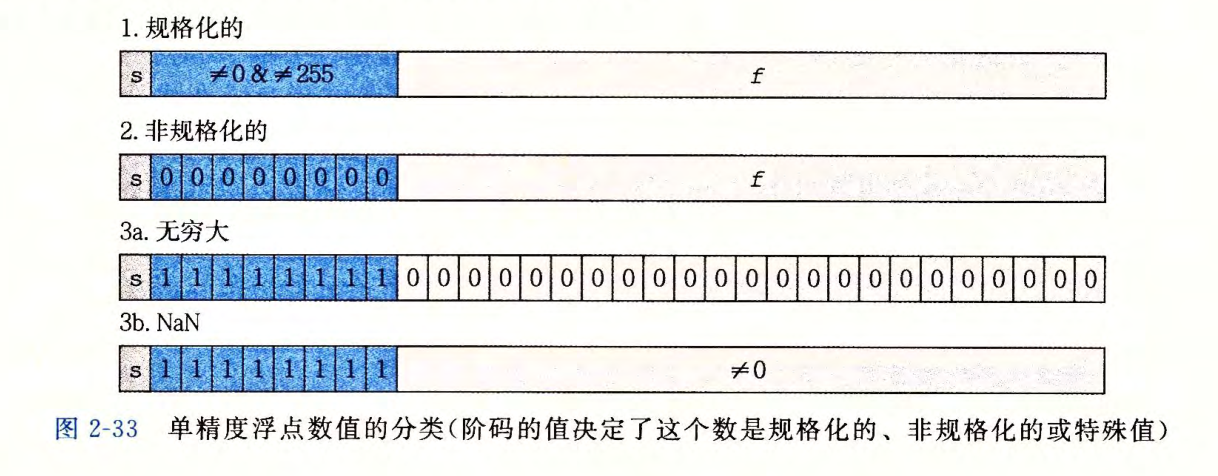
\includegraphics[height=4cm]{QQ20250920-082456}
		\end{center}
		此图来自深入理解计算机系统 (Randal E. Bryant, David R. O’Hallaron) (Z-Library) \\
		
	\end{solution}
	
\end{document}